\documentclass[../../main.tex]{subfiles}

\begin{document}

\chapter{Projections}\label{chap:projections}

Projection operators provide a mathematical framework for decomposing vectors into components along different subspaces, which is essential for understanding least squares problems, orthogonal decompositions, and many iterative methods.

\section{Notation and Setup}\label{sec:projections-notation}
\begin{description}[style=nextline, labelwidth=5cm, leftmargin=5.5cm, font=\normalfont\bfseries]
    \item[Linear system.] Solve \(A\mathbf{x}=\mathbf{b}\) with \(A \in \mathbb{R}^{n\times n}\), \(\mathbf{x},\mathbf{b} \in \mathbb{R}^n\). The exact solution is \(\mathbf{x}^{\ast}  = A^{-1}\mathbf{b}\) (when \(A\) is nonsingular).
    \item[Initial guess.] \(\mathbf{x}_0 \in \mathbb{R}^n\).
    \item[Residuals.] Given \(\mathbf{x}_0\), the current residual is \(\mathbf{r} = \mathbf{b} - A \mathbf{x}\), and the initial residual is \(\mathbf{r}_0 = \mathbf{b} - A \mathbf{x}_0\).
    \item[Subspaces.]
          \begin{itemize}
              \item \emph{Search space} \(\mathcal{K}\subset\mathbb{R}^n\) of dimension \(m\).
              \item \emph{Constraint (left) space} \(\mathcal{L}\subset\mathbb{R}^n\) of dimension \(m\).
          \end{itemize}

    \item[Bases / matrices.]
          \begin{itemize}
              \item \(V=[\mathbf{v}_1,\dots,\mathbf{v}_m] \in \mathbb{R}^{n\times m}\) with \(\mathrm{range}(V)=\mathcal{K}\).
              \item \(W=[\mathbf{w}_1,\dots,\mathbf{w}_m] \in \mathbb{R}^{n\times m}\) with \(\mathrm{range}(W)=\mathcal{L}\).
              \item Unless stated otherwise, \(V\) and \(W\) have full column rank.
          \end{itemize}
    \item[Trial solution.] \(\mathbf{x} = \mathbf{x}_0 + V\mathbf{y}\) with coefficients \(y \in \mathbb{R}^m\).
    \item[Petrov--Galerkin condition.] The residual is orthogonal to \(\mathcal{L}\):
          \[
              \mathbf{r} \perp \mathcal{L} \quad \Longleftrightarrow \quad W^{\top} \left(\mathbf{b}-A(\mathbf{x}_0+V\mathbf{y})\right) = 0.
          \]
          This yields the reduced (\(m \times m\)) system
          \[
              H \mathbf{y} =\mathbf{g}, \qquad H :=W^{\top}AV, \quad \mathbf{g} := W^{\top} \mathbf{r}_0,
          \]
          and the update \(\mathbf{x}=\mathbf{x}_0+V\mathbf{y}\).
          The matrix \(H\) must be nonsingular for \(y\) to be uniquely defined.
    \item[Orthogonal projections.] \(\mathcal{L}=\mathcal{K}\) \(\Rightarrow\) condition \(V^T\mathbf{r}=0\).
    \item[Oblique projections.] \(\mathcal{L}\neq\mathcal{K}\) (e.g.\ \(\mathcal{L}=A\mathcal{K}\)) \(\Rightarrow\) condition \(W^{\top}\mathbf{r}=0\) with a different left basis.
    \item[Projectors (Euclidean).] For a full-rank basis \(B \in \mathbb{R}^{n\times m}\),
          \[
              P_{\mathrm{range}(B)} := B(B^TB)^{-1}B^{\top},
          \]
          and if \(B\) has orthonormal columns, \(P_{\mathrm{range}(B)}=BB^{\top}\).
    \item[$A$-inner product.] If \(A\) is symmetric positive definite (SPD), define the \(A\)-inner product \((\mathbf{u},\mathbf{v})_A:=\mathbf{u}^{\top} A \mathbf{v}\) and the energy norm \(\|\mathbf{u}\|_A:=\sqrt{\mathbf{u}^{\top} A \mathbf{u}}\).
    \item[Special choices.]
          \begin{itemize}
              \item \(\mathcal{L}=\mathcal{K}\) (Galerkin, SPD \(A\)): best approximation in \(\|\cdot\|_A\).
              \item \(\mathcal{L}=A\mathcal{K}\) (residual minimization): best approximation in residual 2-norm.
          \end{itemize}
\end{description}

\section{Projection Operator}\label{sec:projection-operator}
A projection finds the \emph{closest point/shadow} of a vector onto a subspace. This operation decomposes any vector into two parts: one lying within the target subspace and another orthogonal to it.

\begin{definition}{Projection Operator}{projection-operator}
    A linear operator $P: V \to V$ on an inner product space $V$ is called a \emph{projection} if it is idempotent:
    \[
        P^2 = P
    \]
\end{definition}

\begin{corollary}{Orthogonal Projection}{orthogonal-projection}
The operator $P$ is called an \emph{orthogonal projection} if it is additionally \emph{self-adjoint/Hermitian}:
\[
    P^H = P
\]
\end{corollary}

The idempotent property captures the essential characteristic of projections: applying the projection twice gives the same result as applying it once. Geometrically, once a vector is projected onto a subspace, further projections leave it unchanged.

\subsection{Properties of Projections}\label{subsec:properties-of-projections}
Let $P$ be a projection operator on an inner product space $V$. Then:
\begin{enumerate}
    \item $\text{Range}(P) = \{v  \in  V : P\mathbf{v} = v\}$ (the range consists of fixed points)
    \item $V = \text{Range}(P) \oplus \text{Null}(P)$ (direct sum decomposition)
    \item If $P$ is an orthogonal projection, then $\text{Range}(P) \perp \text{Null}(P)$
    \item The eigenvalues of any projection are 0 and 1
\end{enumerate}
\begin{proof}
    \begin{enumerate}
        \item If $\mathbf{v} \in \text{Range}(P)$, then $\mathbf{v} = Pu$ for some $u$, so $P\mathbf{v} = P^2u = Pu = v$. Conversely, if $P\mathbf{v} = v$, then $v$ is clearly in the range of $P$.
        \item For any $\mathbf{v} \in V$, write $\mathbf{v} = P\mathbf{v} + (\mathbf{v} - P\mathbf{v})$. Since $P\mathbf{v}  \in  \text{Range}(P)$ and $P(\mathbf{v} - P\mathbf{v}) = P\mathbf{v} - P^2 \mathbf{v} = P\mathbf{v} - P\mathbf{v} = 0$, we have $\mathbf{v} - P\mathbf{v}  \in  \text{Null}(P)$.
        \item For orthogonal projections, if $u  \in  \text{Range}(P)$ and $v  \in  \text{Null}(P)$, then $\mathbf{u} =P\mathbf{w}$ for some $w$, and $\langle u, \mathbf{v} \rangle = \langle P\mathbf{w}, \mathbf{v} \rangle = \langle \mathbf{w}, P^{\ast} \mathbf{v} \rangle = \langle \mathbf{w}, P\mathbf{v} \rangle = \langle \mathbf{w}, 0 \rangle = 0$.
        \item The eigenvalues of any projection are 0 and 1, since $P^2 = P$ implies the minimal polynomial divides $\mathbf{x}(\mathbf{x}-1)$, so the only possible eigenvalues are 0 and 1.
    \end{enumerate}
\end{proof}

\begin{figure}[ht]
    \centering
    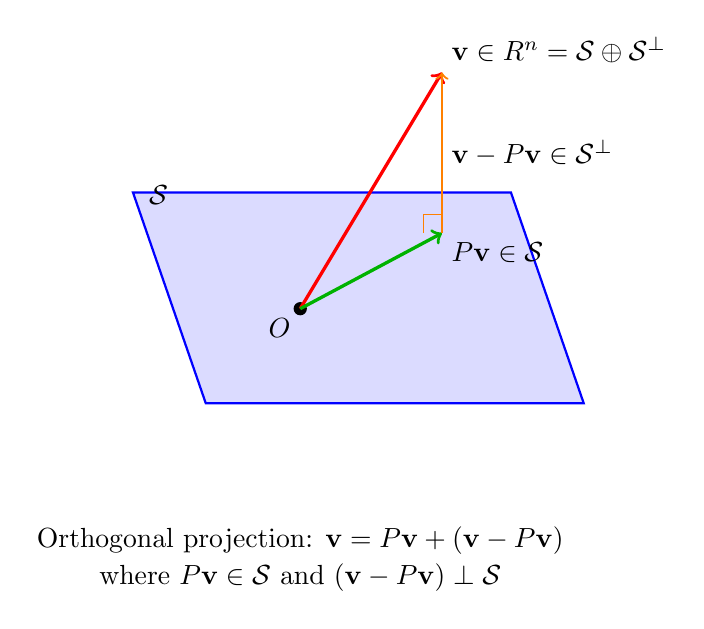
\begin{tikzpicture}[scale=1.2]
    % Draw the subspace S (as a 3D plane)
    \fill[blue!20, opacity=0.7] (-1,-1,0) -- (3,-1,0) -- (3,2,2) -- (-1,2,2) -- cycle;
    \draw[blue, thick] (-1,-1,0) -- (3,-1,0) -- (3,2,2) -- (-1,2,2) -- cycle;

    % Origin
    \fill[black] (0,0) circle (2pt);
    \node[below left] at (0,0) {$O$};

    % Original vector v
    \draw[red, very thick, ->] (0,0) -- (1.5,2.5);
    \node[above right] at (1.5,2.5) {$\mathbf{v} \in \mathbb{R}^n = \mathcal{S} \oplus \mathcal{S}^\perp$};

    % Projection Pv onto the subspace
    \draw[green!70!black, very thick, ->] (0,0) -- (1.5,0.8);
    \node[below right] at (1.5,0.8) {$P\mathbf{v} \in \mathcal{S}$};

    % Orthogonal component (v - Pv)
    \draw[orange, thick, ->] (1.5,0.8) -- (1.5,2.5);
    \node[right] at (1.5,1.65) {$\mathbf{v} - P\mathbf{v} \in \mathcal{S}^\perp$};

    % Perpendicular indicator
    \draw[orange, thin] (1.3,0.8) -- (1.3,1.0) -- (1.5,1.0);

    % Subspace label
    \node at (-1.5,1.2) {$\mathcal{S}$};

    % Annotation
    \node[below] at (0,-2.2) {Orthogonal projection: $\mathbf{v} = P\mathbf{v} + (\mathbf{v} - P\mathbf{v})$};
    \node[below] at (0,-2.6) {where $P\mathbf{v} \in \mathcal{S}$ and $(\mathbf{v} - P\mathbf{v}) \perp \mathcal{S}$};
\end{tikzpicture}

    \caption{Geometric interpretation of orthogonal projection. The vector $v$ is decomposed into its projection $P\mathbf{v}$ onto the subspace $S$ and the orthogonal component $\mathbf{v} - P\mathbf{v}$.}
    \label{fig:orthogonal-projection}
\end{figure}

\section{Reduced Systems}\label{sec:reduced-systems}
In iterative methods for solving linear systems, we often work with reduced systems $H$, that capture the essential features of the original problem \eqref{eq:linear-system} within a lower-dimensional subspace.

\begin{proposition}{Galerkin with SPD $A$}{galerkin-spd}
    If $A=A^\top\succ0$ and $\mathcal{L}=\mathcal{K}$, then for any full-rank bases $V,W$ with $\operatorname{range}(V)=\operatorname{range}(W)=\mathcal{K}$, the matrix $H=W^\top A V$ is symmetric positive definite and hence invertible.
\end{proposition}
\begin{proof}[Proof sketch]
    Write $W=VG$ with $G\in\mathbb{R}^{m\times m}$ invertible. Then $H=G^\top V^\top A V$. Since $A=C^\top C$ and $V$ has full column rank, $V^\top A V=(CV)^\top(CV)\succ0$.
\end{proof}

\begin{proposition}{Petrov--Galerkin with $\mathcal{L}=A\mathcal{K}$}{petrov-ak}
    Suppose $A$ is invertible and $\mathcal{L}=A\mathcal{K}$. For full-rank $V$ with $\operatorname{range}(V)=\mathcal{K}$, choose $W=AVG$ with $G$ invertible. Then $H=W^\top A V = G^\top (AV)^\top(AV)\succ0$ and is invertible.
\end{proposition}

These conditions underpin the optimality results: Galerkin ($\mathcal{L}=\mathcal{K}$) yields best approximation in the $A$-norm when $A\succ0$, while $\mathcal{L}=A\mathcal{K}$ yields residual 2-norm minimization.

\section{Matrix Representation of Projections}\label{sec:matrix-representation-of-projections}

In finite-dimensional spaces, projections can be represented as matrices with specific structural properties.

\begin{theorem}{Matrix Characterization of Orthogonal Projections}{matrix-projection}
    A matrix $P  \in  \mathbb{R}^{n \times n}$ represents an orthogonal projection if and only if:
    \begin{enumerate}
        \item $P^2 = P$ (idempotent)
        \item $P^{\top} = P$ (symmetric)
    \end{enumerate}
    In this case, $P$ projects onto $\text{Col}(P)$ along $\text{Null}(P)$.
\end{theorem}

The geometric interpretation is crucial: $P$ maps every vector to its closest point in the column space of $P$, measured in the Euclidean norm.

\begin{example}{Simple Projection Examples}{simple-projections}
    \textbf{Projection onto a line:} Let $u  \in  \mathbb{R}^n$ be a unit vector. The projection onto the line spanned by $u$ is:
    \[
        P_u = uu^{\top}
    \]

    \textbf{Projection onto coordinate subspace:} The projection onto the first $k$ coordinates is:
    \[
        P_k = \begin{pmatrix} I_k & 0 \\ 0 & 0 \end{pmatrix}
    \]
    where $I_k$ is the $k \times k$ identity matrix.
\end{example}

\section{Oblique Projections}\label{sec:oblique-projections}

Not all useful projections are orthogonal. An \emph{oblique} projection maps onto a target subspace along a (non-orthogonal) complementary subspace.

\begin{definition}{Oblique Projection}{oblique-projection}
    Let $\mathcal{S},\mathcal{T} \subset\mathbb R^n$ be subspaces with a direct sum decomposition

    \begin{align*}
        \mathbb R^n                & =\mathcal{S}\oplus\mathcal{T} \\
        \mathcal{S}\cap\mathcal{T} & =\{0\}
    \end{align*}

    The \emph{oblique projection} $P$ onto $\mathcal{S}$ along $\mathcal{T}$ is the unique linear map
    satisfying $\mathrm{range}(P)=\mathcal{S}$ and $\mathrm{null}(P)=\mathcal{T}$; equivalently,
    \[
        P\mathbf v\in\mathcal{S},\qquad \mathbf v-P\mathbf v\in\mathcal{T},\qquad \forall\,\mathbf v\in\mathbb{R}^n
    \]
\end{definition}

\paragraph{Matrix realizations:}
Let $S\in\mathbb R^{n\times k}$ have full column rank with $\mathrm{range}(S)=\mathcal{S}$.
\begin{itemize}
    \item If $W\in\mathbb R^{n\times k}$ has full column rank with $\ker(W^\top)=\mathcal{T}$ (i.e., $\mathrm{range}(W)=\mathcal{T}^\perp$) and $W^\top S$ is nonsingular, then
          \[
              P=S(W^\top S)^{-1}W^\top
          \]
          This realizes the projector \emph{onto $\mathcal{S}$ along $\mathcal{T}$}. (Note: using $T^\top$ in place of $W^\top$ would project along $\mathcal{T}^\perp$, not along $\mathcal{T}$.)
    \item If $T\in\mathbb R^{n\times(n-k)}$ spans $\mathcal{T}$ and the block $[S\ T]$ is invertible, then
          \[
              P=[ST]
              \begin{bmatrix}
                  I_k & 0 \\
                  0   & 0
              \end{bmatrix}
              [ST]^{-1}.
          \]
\end{itemize}
In general $P$ is not symmetric ($P^\top\neq P$) but is always idempotent ($P^2=P$).

\begin{example}{Oblique projection in iterative methods}{oblique-projection-iterative}
    In iterative solvers for $A\mathbf x=\mathbf b$, choose a \emph{search space} $\mathcal K=\mathrm{span}(V)$
    and a \emph{test space} $\mathrm{span}(W)$; the Petrov--Galerkin condition $W^\top\mathbf r=0$ produces
    \[
        P=V(W^\top V)^{-1}W^\top,
    \]
    which is the oblique projector onto $\mathcal K$ along $\ker(W^\top)$.

    With $W$ chosen so that $\mathrm{span}(W)=A\mathcal K$ (as in GMRES), the residual is enforced orthogonal to $A\mathcal K$, i.e., the projection is along $(A\mathcal K)^\perp$.
\end{example}

\begin{figure}[htb]
    \centering
    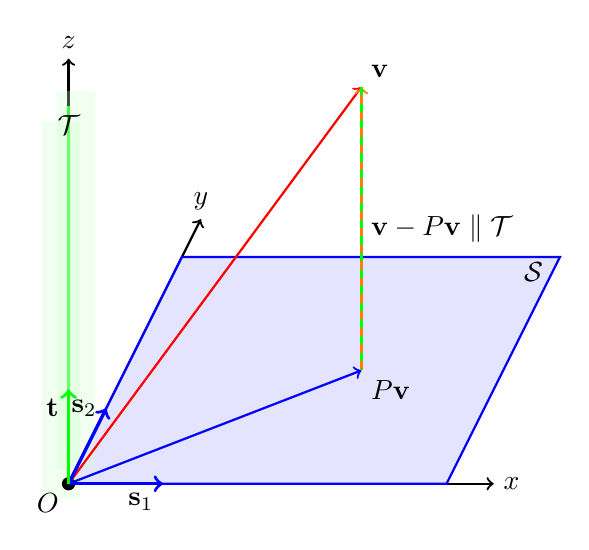
\begin{tikzpicture}[scale=1.2]
    % Set up 3D coordinate system with better perspective
    \begin{scope}[x={(1cm,0cm)}, y={(0.4cm,0.8cm)}, z={(0cm,1cm)}]

        % Add coordinate axes for reference
        \draw[thick, ->] (0,0,0) -- (4.5,0,0);
        \draw[thick, ->] (0,0,0) -- (0,3.5,0);
        \draw[thick, ->] (0,0,0) -- (0,0,4.5);
        \node[right] at (4.5,0,0) {$x$};
        \node[above] at (0,3.5,0) {$y$};
        \node[above] at (0,0,4.5) {$z$};

        % Draw the projection space (S) - a plane
        \fill[blue!15, opacity=0.7] (0,0,0) -- (4,0,0) -- (4,3,0) -- (0,3,0) -- cycle;
        \draw[blue, thick] (0,0,0) -- (4,0,0) -- (4,3,0) -- (0,3,0) -- cycle;

        % Draw the oblique direction space (T) - a line through origin
        \draw[green, thick] (0,0,0) -- (0,0,4);
        \fill[green!20, opacity=0.3] (-0.2,-0.2,0) -- (0.2,-0.2,0) -- (0.2,-0.2,4) -- (-0.2,-0.2,4) -- cycle;
        \fill[green!20, opacity=0.3] (-0.2,0.2,0) -- (0.2,0.2,0) -- (0.2,0.2,4) -- (-0.2,0.2,4) -- cycle;

        % Origin
        \fill[black] (0,0,0) circle (2pt);
        \node[below left] at (0,0,0) {$O$};

        % Original vector v (outside both spaces)
        \draw[red, thick, ->] (0,0,0) -- (2.5,1.5,3);
        \node[above right] at (2.5,1.5,3) {$\mathbf{v}$};

        % Projection Pv onto S along T
        \draw[blue, thick, ->] (0,0,0) -- (2.5,1.5,0);
        \node[below right] at (2.5,1.5,0) {$P\mathbf{v}$};

        % Residual vector (v - Pv) - parallel to T
        \draw[orange,thick, ->] (2.5,1.5,0) -- (2.5,1.5,3);
        \node[right] at (2.5,1.5,1.5) {$\mathbf{v} - P\mathbf{v} \parallel \mathcal{T}$};

        % Show the oblique projection line (parallel to T)
        \draw[green, dashed, thick] (2.5,1.5,3) -- (2.5,1.5,0);

        % Basis vectors for S (projection space)
        \draw[blue, very thick, ->] (0,0,0) -- (1,0,0);
        \node[below left] at (1,0,0) {$\mathbf{s}_1$};
        \draw[blue, very thick, ->] (0,0,0) -- (0,1,0);
        \node[left] at (0,1,0) {$\mathbf{s}_2$};

        % Direction vector for oblique projection (spanning T)
        \draw[green,very thick, ->] (0,0,0) -- (0,0,1);
        \node[below left] at (0,0,1.0) {$\mathbf{t}$};

        % Labels for subspaces with better positioning
        \node at (3.8,2.8,0) {$\mathcal{S}$};
        \node at (0,0,3.8) {$\mathcal{T}$};
    \end{scope}
\end{tikzpicture}

    \caption{Oblique projection: \(P\mathbf{v}\in\mathcal{S},\ \mathbf{v}-P\mathbf{v}\in\mathcal{T}\) (not necessarily orthogonal). Basis vectors \(\mathbf{s} \in \mathcal{S}\) and \(\mathbf{t} \in \mathcal{T}\) are shown.}
    \label{fig:oblique-projection}
\end{figure}

\end{document}